\documentclass[11pt,a4paper]{article}

\usepackage{graphicx}
\graphicspath{ { ./img/ } }
\usepackage[margin=1in]{geometry}
\usepackage{url}
\usepackage{xcolor}
\usepackage{algpseudocode}
\usepackage{url}

\title{\textbf{CS142 Coursework II}}
\author{Artemy Bulavin \\ 1812276}
\date{}

\begin{document}

\maketitle
% A summary of your research
% A description of the algorithm/data set/system you are visualising
% A description of the process/techniques you have used to visualise it
% A justification of the visual choices you have made
% An image/set of images showing the output – you might also want to 
% include images of early work in progress
% A reflection on how effective the visualisation is

% MARKING CRITERIA:
% Well written and shows evidence of sufficient research into the topic
% Demonstrates that you have considered what makes a good visualisation
% Shows a critical reflection on the final output
% Well structured and well formatted
% Includes comprehensive and relevant references to your research and
% to your sources of inspiration.

\section*{Introduction}
\hrule
\vspace{11pt}
The aim of this visualisation is to demonstrate the process of Dijkstra's Shortest Path algorithm using 
a simple graph with weighted edges, where colours of vertices and edges change based on the different stages
of the algorithm.

\section*{Dijkstra's Shortest Path Algorithm}

Dijkstra's Shortest Path algorithm is a method for finding the shortest distance from a given
source node to all other nodes in a simple, weighted graph \cite{djikstra1959note}. The version of the algorithm
used in this visualisation is the original version, as opposed to min-priority queue implementation \cite{fredman1987fibonacci}.
\\
\\
The algorithm works as follows:
\begin{enumerate}
	\item Mark all nodes as unvisited and construct a set of all unvisited nodes.
	\item Give the source node a tentative distance of 0, and all other nodes a tentative distance of $\infty$.
	\item For the current node, calculate the tentative distance from the current node to its adjacent neighbours.
	Compare this distance to the distance already assigned to the node and choose the minimum of the two to be
	the node's tentative distance.
	\item Once all neighbours of current node have been considered, mark it as visited and remove it from the
	unvisited set. Visited nodes are not visited again.
	\item If the unvisited set is empty, the algorithm ends.
	\item Choose the next current node from the unvisited set to be the one with the smallest tentative distance.
	Go to step 3.
\end{enumerate}
\newpage
\noindent
The algorithm is implemented using the following pseudocode \cite{wiki:code}.
\\
\begin{algorithmic}
\Function{dijkstra}{Graph $G$, source}

\State Create vertex set $Q$ from $G$
\ForAll{Vertex $v$ in $Q$}
\State distance[$v$] $\leftarrow \infty$
\State previous[$v$] $\leftarrow$ null 
\EndFor
\State distance[source] $\leftarrow 0$
\While{Q is not empty}
\State $u \leftarrow$ vertex with smallest distance[u]
\State Remove $u$ from $Q$
\ForAll{neighbours $v$ of $u$}
\State newDistance $\leftarrow$ dist[$v$] + length($u,v$)
\If{newDistance $<$ dist[$v$]}
\State dist[$v$] $\leftarrow$ newDistance
\State previous[$v$] $\leftarrow u$ 
\EndIf
\EndFor
\EndWhile
\\
\Return distance, previous
\EndFunction
\end{algorithmic}

\section*{Design and Implementation}

The algorithm would be visualised using a simple, connected graph with weighted edges that are positioned
isometrically so that the distances between adjacent nodes are equal for all nodes. This is so that edges between
nodes are not tangled (especially for larger graphs) and the graph is visually penetrable \cite{card1999readings}.
Since the nodes are arbitrary
their position in the space does not convey any information. This means the system by which the nodes are placed
in the space needs to be decided \cite{mazza2009introduction}. In order to achieve the best layout
and allow for maximum visual penetration, isometric spacing was chosen.

\subsection*{Drawing Vertices}

In order to achieve this, \texttt{Node} and \texttt{Edge} classes were created that would form the structure
of the graph. These were encapsulated further by a \texttt{Graph} class that would handle graph generation and
drawing of the nodes and edges.
\\
Each vertex of the graph contains a \texttt{PVector} representing the location of the vertex. During
\texttt{generateGraph()} in class \texttt{Graph}, $n$ vertices are created, where $n$ is the number of points. Each vertex is given an $x$ and $y$ value that ensure isometric positioning,
For each vertex a \texttt{button} object is also created using the ControlP5 class to allow for interaction later.
\\
The space between each vertex is ultimately determined by the variable \texttt{scale}, which is calculated from
the number of points and screen dimensions to ensure that for any number of points, the graph scales to fit the
space.
\\
This allowed for any number of points to be drawn as an isometric grid (Figure \ref{1}).
\newpage
\begin{figure}[h]
	\centering
	\caption{Initial Vertex positioning}
	\vspace{10pt}
	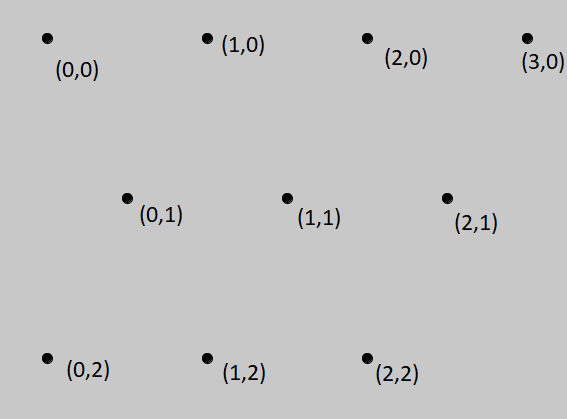
\includegraphics[scale=0.5]{graph1.png}
	\label{1}
\end{figure}
\noindent

\subsection*{Drawing Edges}

Next, the edges would have to be drawn between each node. To do this, a matrix representation of the graph 
is created using a 2D array that assigns each node to a row and column (Figure \ref{1}). This allowed for
rules to be established that determined how the nodes would be connected to each other.
\\
For a node in the matrix with position $(i,j)$ where $i$ is the column and $j$ is the row:
\begin{itemize}
	\item If a node is in the top row i.e $j = 0$ then create an edge to 
	$(i+1,j)$ and $(i,j+1)$.
	\item If a node is on the bottom row and is on an \emph{even} row  i.e $j \pmod $ $2 \equiv 0$,
	then create an edge to $(i+1,j)$ and $(i,j-1)$. If it's on an odd row, create an edge to $(i+1,j-1)$
	and $(i+1,j)$.
	\item Otherwise, if the vertex is not on the top or bottom row, and is on an even row then create an edge to
	$(i,j-1)$, $(i,j+1)$ and $(i+1,j)$. If it's on an odd row, then create edges to $(i+1,j-1)$, $(i+1,j)$ and $(i+1,j+1)$.
\end{itemize}
Each \texttt{Edge} object created is also assigned a random weight between 30 and 110 inclusive. This is so that
there is enough variation in the weights of the edges for the algorithm to illustrate paths between nodes that
were not intuitive or apparent immediately.
\\
This allowed for an almost complete graph to be drawn, with drawn edges on the screen corresponding to edges in
the Graph data structure (Figure \ref{2}).
\begin{figure}[h]
	\centering
	\caption{Edges Added}
	\vspace{10pt}
	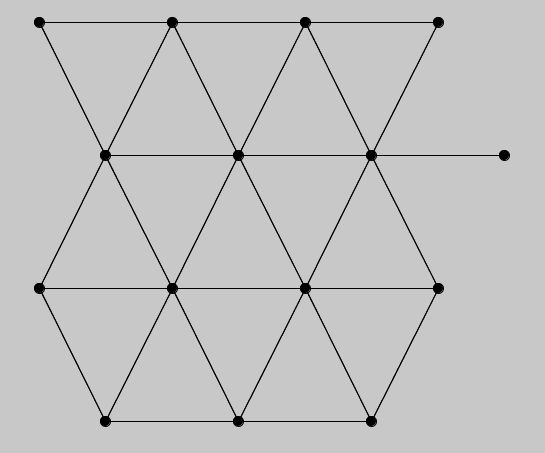
\includegraphics[scale=0.5]{graph2.png}
	\label{2}
\end{figure}

\subsection*{Labelling}

In order to label vertices, each vertex has a letter A-Z assigned to it that is drawn directly above.
While the labels are redundant in the sense that they are not necessary for the algorithm, their change in colour of the
labels helps to illustrate the current stage of the algorithm.
Vertices are also coloured based on whether they are the current vertex, have been visited or remain unvisited. This is done
using the \texttt{State} enumeration. The current vertex is drawn in yellow, visited vertices and edges in green and
unvisited vertices in magenta purple. The colours are chosen to accommodate for red-green colour-blindness - the yellow provides 
enough distinction from the magenta and green, and the magenta will not appear similar to the green \cite{wong2011points}.
\\
\\
In order to label edges, the weight of the edge is drawn by the line as a number. While Mazza \cite{mazza2009introduction}
suggests to use line thickness/weight or labels for edge weight, line thickness is a pre-attentive attribute that conveys
quantitative information poorly in this case. For example, two edge, one with eight 63 and another with 70 may appear almost
identical to the viewer, meaning that once the resulting shortest path is displayed it cannot easily be verified by checking
the weights of the edges in the path. Therefore, while adding extra text to the visualisation may require the viewer
to mentally maintain numbers in their working memory and draw attention away from the algorithm \cite{tufte}, this is preferred
for when the algorithm ends and the viewer can interact with and verify the shortest paths themselves.
\\
\\
With the added labels and colours, the algorithm is ready to be animated (Figure \ref{3}).
\begin{figure}[h]
	\centering
	\caption{Edges Added}
	\vspace{10pt}
	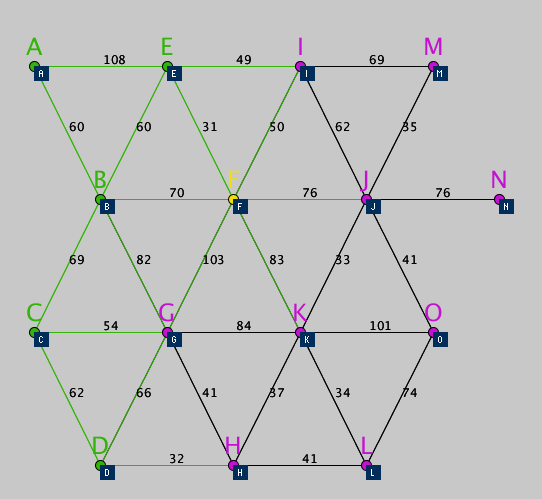
\includegraphics[scale=0.6]{graph3.png}
	\label{3}
\end{figure}

\subsection*{Animation}

\newpage
\bibliographystyle{plain}
\bibliography{ref}


\end{document}